 % Niveau :      PCSI - PC
% Discipline :  Elec
% Mots clés :   Elec, Ordre 2

\begin{exercise}{Bobine réelle}{1}{Sup,Spé}
{\'Electrocinétique, Circuits d'ordre 2}{lelay,centrale}

Dans cet exercice, on cherche à étudier les caractéristique d'une bobine réelle (par opposition à une bobine idéale).

\begin{questions}
    \questioncours Composants élémentaires en électrocinétique et ordres de grandeur.
    \question En quoi consiste une bobine réelle (dans la vraie vie, par opposition à bobine "idéale") ? Justifier qu'on représente une bobine réelle par une bobine parfaite et une résistance en série.
    \question On s'intéresse au circuit suivant. A l'aide d'une étude asymptotique, trouver quel filtre est ici réalisé.

\begin{circuit}
      \draw
      node [ground] at (0,0) {}
      (0,0) to [sV, v^>=$U_e$] (0,2)
            to [R, l=$r$] (2,2)
            to [L, l=$L$] (4,2)
            to [C, l=$C$] (6,2)
            to [R, l_=$R$, v^<=$U_s$] (6,0)
            to [short]    (0,0);
      \draw [red, dashed] (0.2,1.5) rectangle(3.8,2.8) ;
      \node [red] at (2.0,3.1) {Bobine réelle};
\end{circuit}
    
    \question Sur l'écran d'un oscilloscope mesurant $U_s$ et $U_e$ on voit le graphe représenté ci dessous. Quelle est la fréquence de ces signaux ? Quel est leur décalage en amplitude ? En phase ?

\begin{figure}[H]
    \centering
    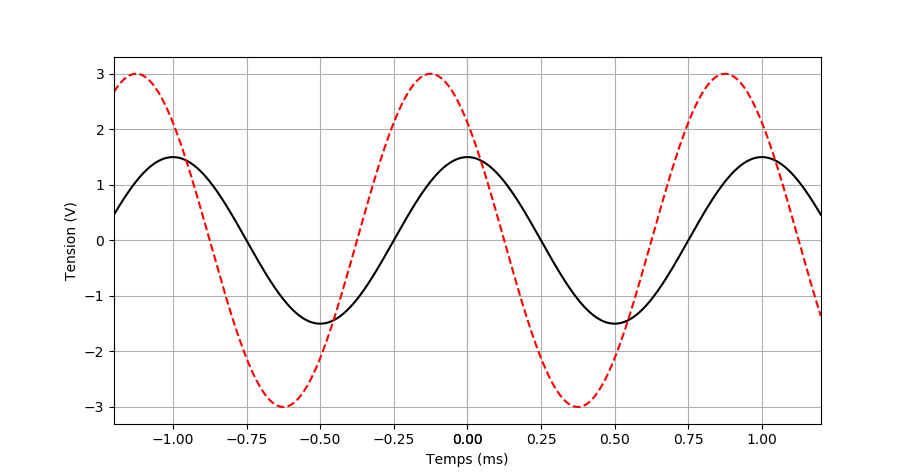
\includegraphics[width=\linewidth]{elec/filtragelineaire/OSCILLO_DECALE.png}
    \caption{En rouge et en tirets : $U_e$ (l'excitation), en noir : $U_s$ (la réponse).}
\end{figure}

    \question Sachant qu'on sait que $C = 1.00$ $\mu$F et $R =1.00$ k$\Omega$, donner la valeur de $L$ et de $r$. Conclure sur la qualité de la bobine utilisée.
\end{questions}
\end{exercise}

\begin{solution}

\begin{questions}
    \questioncours Parler un peu de C et L en vrai, OdG genre 1 nF et 10 mH
    \question C'est un long fil donc normal résistance
    \question Passe-bande
    \question Fréquence : $\omega = 1 kHz$, décalage en amplitude : facteur 1/2, décalage en fréquence : -pi/4 donc $H(\omega) = \frac12e^{-i\pi/4}$
    \question La fonction de transfert est bien sur $H(\omega) = \frac1{1+\frac{r}R + j\frac1R\qty(L\omega-\frac{1}{C\omega})}$. On utilise la phase d'abord : 
    \begin{align*}
    arg\qty(\frac1{1+\frac{r}R + j\frac1R\qty(L\omega-\frac{1}{C\omega})}) = -arg\qty( 1+\frac{r}R + j\frac1R\qty(L\omega-\frac{1}{C\omega}) ) = -\frac{\pi}4 \\
    \arctan\qty(\frac{\frac1R\qty(L\omega-\frac{1}{C\omega})}{1+\frac{r}R}) = \frac{\pi}4 \\
    \frac{\frac1R\qty(L\omega-\frac{1}{C\omega})}{1+\frac{r}R} = 1 \\
    \frac1R\qty(L\omega-\frac{1}{C\omega}) = 1+\frac{r}R
    \end{align*}
    Ensuite, l'amplitude :
    \begin{align*}
    \abs{\frac1{1+\frac{r}R + j\frac1R\qty(L\omega-\frac{1}{C\omega})}} = \frac1{\abs{1+\frac{r}R + j\frac1R\qty(L\omega-\frac{1}{C\omega})}} = \frac12\\
    \abs{1+\frac{r}R + j\frac1R\qty(L\omega-\frac{1}{C\omega})} = 2 \\
    \sqrt{\qty(1+\frac{r}R)^2 + \frac1R\qty(L\omega-\frac{1}{C\omega})^2} = 2
    \end{align*}
    On utilise le résultat sur la phase
    \begin{align*}
    \sqrt{2}\qty(1+\frac{r}R) = 2 \\
    1+\frac{r}R = \sqrt{2} \\
    r = R(\sqrt{2} -1)
    \end{align*}
    Et on repart du résultat sur la phase
    \begin{align*}
    \frac1R\qty(L\omega-\frac{1}{C\omega}) = \sqrt{2} \\
    L = \frac{R\sqrt{2}}{\omega} + \frac1{C\omega^2}
    \end{align*}
    Donc voilà
    
\end{questions}

\end{solution}
